\documentclass[../main.tex]{subfiles}

\begin{document}
\subsection*{Exercice 1 : Forme canonique et poursuite de trajectoire}
\begin{enumerate}

\item

\begin{enumerate}
\item
On a toujours le système suivant : \[\left \{ \begin{matrix}
\dot{x_1} &= &\begin{pmatrix}-10&12\\-6&7\end{pmatrix} x_1 &+ \begin{pmatrix}-1\\-1\end{pmatrix}u\\
y_1 &= &\begin{pmatrix}4&-5\end{pmatrix}x_1
\end{matrix} \right.\]
Et on a effectué le changement de variable suivant : $x_1(t) = Mx_c(t)  x_c = \begin{pmatrix}z_1\\z_2\end{pmatrix}$
On a donc le système équivalent :
\[\left \{ \begin{matrix}
\dot{x_c} &= &\begin{pmatrix}0&1\\-2&-3\end{pmatrix} x_c &+ \begin{pmatrix}0\\-1\end{pmatrix}u\\
y &= &\begin{pmatrix}0&1\end{pmatrix}x_c
\end{matrix} \right.\]
\item On impose la trajectoire :
\begin{align*}
y_d(t) &= 10\left(\frac{t}{T}\right)^3 - 15\left(\frac{t}{T}\right)^4 + 6\left(\frac{t}{T}\right)^5
\intertext{Le système est équivalent à :}
\text{avec l'équation d'observation : }& y(t) = z_2(t)\\
\text{et le système d"état donne : }&\left\{\begin{matrix}
\dot{z_2} = -2z_1-3z_2+u\\
\dot{z_1} = z_2
\end{matrix}\right.
\intertext{Et comme on impose la trajectoire sur $y(t) = y_d(t)$, on a :}
z_2^d(t) &= y_d(t)
\intertext{donc $z_1^d(t)$ doit vérifier :}
z_1^d(t) &= \int_0^t y_d(\tau) d\tau\\
 &= \frac{10T}{4}\left(\frac{t}{T}\right)^4 - \frac{15T}{5}\left(\frac{t}{T}\right)^5 + \frac{6T}{6}\left(\frac{t}{T}\right)^6
\end{align*}
\item  On note :
\begin{align*}
\epsilon_d(t) &= z_1(t) - z_1^d(t)
\intertext{On cherche a déterminer le vecteur de la formule de Bumowski qui annulera $\epsilon_d(t)$}
v(t) &= -a^Tx_c(t) + u(t) \text{	avec, }a=\begin{pmatrix}2&3\end{pmatrix}\\
&\left\{\begin{matrix}
\dot{z_1}=z_2\\
\dot{z_2}=v
\end{matrix}\right. \Rightarrow v = \ddot{z_1}\\
\ddot{\epsilon_d} &= \ddot{z_1}-\ddot{z_1^d}\\
&= v - \ddot{z_1^d}
\end{align*}
On cherche donc à avoir $\epsilon_d(t)$ solution de $\ddot{\epsilon_d}(t) + h_1 \dot{\epsilon_d}(t) + h_0 \epsilon_d(t) = 0$, où $(h_0,h_1) \in \mathbb{R}^2$ à déterminer et dépendant du vecteur v. Tel que l'équation caractéristique possède des racines à parties réelles négatives. Donc ssi $h_1>0$ et $h_0>0$.\\
La transformée de Laplace de cette équation donne donc :
\begin{align*}
p^2\epsilon_d(p) &- p\epsilon_d(0^+) - \dot{\epsilon_d}(0^+) + h_1(p\epsilon_d - \epsilon_d(o^+))+ h_0\epsilon_d(p) = 0\\
\epsilon_d &= \frac{\dot{\epsilon_d}(0^+)+(h_1+p)\epsilon_d(0^+)}{p^2+h_1p + h_0}\\
&=\frac{\gamma_1p+\gamma_0}{(p-p_1)(p-p_2)}
\end{align*}
Exemple : $p^2+h_1p + h_0 = (p+\frac{10}{T})^2 = p^2 + \frac{20p}{T} + \frac{100}{T^2}$\\

$v$ doit vérifier d'après l'expression de $\ddot{\epsilon_d}$ :
\begin{align*}
v(t) &= \ddot{\epsilon_d}(t) + \ddot{z_1^d}(t)\\
&= \ddot{z_1^d}(t) - h_1(\dot{z_1}(t)-\dot{z_1^d}(t))- h_0(z_1(t) - z_1^d(t))\\
&= \begin{pmatrix}
h_0&h_1\end{pmatrix}.\begin{pmatrix}
z_1\\z_2\end{pmatrix} + (\ddot{z_1^d}(t) + h_1\dot{z_1^d}(t)+ h_0z_1^d(t))\\
&= -Kx_c + \tilde{z_d}
\intertext{or, $v=-a^Tx_c + u$, donc on obtient la loi de commande :}
u &= -Kx_c + \tilde{z_d} + a^Tx_c\\
&= (a^T-K)x_c + \tilde{z_d}
\end{align*}

Loi de commande en BF par retour d'état :
\begin{center}
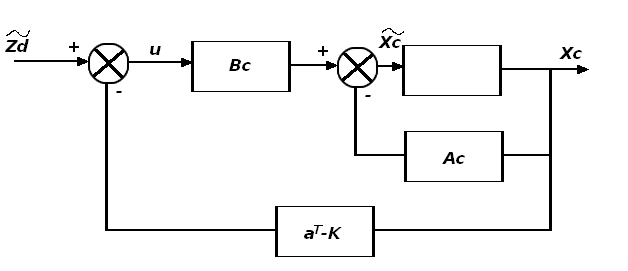
\includegraphics[scale=0.5]{TD8.png}
\end{center}



\end{enumerate}
\end{enumerate}

\subsection*{Exercice 2 : Synthèse d'une loi de commande par retour d'état}
\begin{enumerate}
\item On a ici, n=3. Déterminons la représentation d'état.\\
On a avec la fonction de transfert :\\
\begin{align*}
A(p)Y(p) &= B(p)U(p)\\
\intertext{d'où l'équation dans le domaine temporelle :}
y^{(3)} + 8 y^{(2)} + 17 y^{(1)} + 10y &= u^{(1)} +2u
\intertext{On a donc la forme canonique de commandabilité :}
\dot{x_c} &= \begin{pmatrix}0&1&0\\0&0&1\\-10&-17&-8\end{pmatrix} x_c + \begin{pmatrix}0\\0\\1\end{pmatrix}u\\
&= A_c x_c +B_c u
\intertext{et on a l'equation d'observation :}
y &= \begin{pmatrix}2\\1\\0\end{pmatrix} x_c + 0.u
\end{align*}
Attention : Le u de l'équation d'état et de la fonction de transfert ne sont PAS les mêmes, l'un est un scalaire l'autre un vecteur.\\

On a une forme canonique de commandabilité, donc le système est effectivement commandable. Cependant, l'observabilité n'est pas acquise.\\
La réalisation est observable ssi il n'y a pas de simplification d'un zéro par un pôle. Il suffit donc de vérifier que -2 n'est pas un zéro du numérateur.\\
Une représentation minimal est appelée réalisation d'état.\\

\item On impose pour la boucle fermée :
\[ \left \{ \begin{matrix}
u = -Kx_c + \eta e\\
K = \begin{pmatrix}k_0 & k_1 & k_2\end{pmatrix} \in \mathbb{R^{1x3}}\\
\end{matrix} \right. \]

On a donc pour l'équation d'état :
\begin{align*}
\dot{x_c} &= A_c x_c + B_c u\\
&= (A_c - B_cK)x_c + \eta B_c e\\
&= A_{bf}x_c + \eta B_c e
\intertext{et pour l'éuation d'obersation : }
y = C_c x_c
\end{align*}

\item On impose les racines $P_1/P_2 = -m\omega_0 \pm j \omega_0\sqrt{1-m^2}$, donc on a le polynôme caractéristique : $\frac{p^2}{\omega_0^2} + \frac{2m}{\omega_0}p + 1$\\
Il est nécessaire de spécifier un troisième pôle $p_3 = -\lambda m \omega_0$, avec $\lambda >> 1$, car la système est d'ordre 3. Comment le choisir? Stable, plus rapide que les autres pôles que l'on impose.\\

On a alors le polynôme à imposer :
\begin{align*}
\Pi_d(p) &= (p + \lambda m \omega_0)(p^2 + 2mp + \omega^2)\\
&= p^3 + (2+\lambda)m\omega_0 p^2 + (2\lambda m^2 + 1) \omega^2 p + \lambda m \omega_0^3
\end{align*}

Pour la matrice $A_{bf}$, on a le polynôme caractéristique :
\begin{align*}
P_{A_{bf}} &= det(p\mathbf{1_3} - A_{bf})\\
&=p^3 + (8+k_2)p^2 + (17+k_1)p + (10+k_0)
\end{align*}
Sachant qu'il y a une lien directe entre les coefficients de la matrice compagnon et son polynôme caractéristique.\\
On identifie donc les coefficients des deux polynômes :
\[\left \{ \begin{matrix}
(8+k_2) = (2+\lambda)m\omega_0\\
(17+k_1) = (2\lambda m^2 + 1) \omega^2\\
(10+k_0) = \lambda m \omega_0^3
\end{matrix} \right. \]

\item Erreur statique nulle ssi le gain en p=0 vaut 1 (gain statique unitaire)\\
Or, \[G_{bf}(p) = C_c(p \mathbf{1_3}-A_{bf})^{-1}B_c \eta \]
Donc , \[ \eta = \frac{1}{-C_c(A_c-B-cK)^{-1}B_c}\]
\end{enumerate}

\end{document}
